\documentclass[12pt]{beamer}
\usepackage{../Estilos/BeamerMAF}
\usepackage{../Estilos/ColoresLatex}
\input{../Preambulos/preambulo_Beamer_Dresden_seahorse}

\setbeamercolor{section in foot}{bg=darkspringgreen, fg=white}
\setbeamercolor{subsection in foot}{bg=persianblue, fg=white}
\setbeamercolor{date in foot}{bg=goldenrod, fg=white}

\makeatletter
\setbeamertemplate{footline}
{
\leavevmode%
\hbox{%
\begin{beamercolorbox}[wd=.333333\paperwidth,ht=2.25ex,dp=1ex,center]{section in foot}%
  \usebeamerfont{section in foot} \insertsection
\end{beamercolorbox}%
\begin{beamercolorbox}[wd=.333333\paperwidth,ht=2.25ex,dp=1ex,center]{subsection in foot}%
  \usebeamerfont{subsection in foot}  \insertsubsection
\end{beamercolorbox}%
\begin{beamercolorbox}[wd=.333333\paperwidth,ht=2.25ex,dp=1ex,right]{date in head/foot}%
  \usebeamerfont{date in head/foot} \insertshortdate{} \hspace*{1.5em}
  \insertframenumber{} / \inserttotalframenumber \hspace*{2ex} 
\end{beamercolorbox}}%
\vskip0pt%
}
\makeatother
% \usefonttheme{serif}
\resetcounteronoverlays{saveenumi}

\AtBeginDocument{\RenewCommandCopy\qty\SI}
\ExplSyntaxOn
\msg_redirect_name:nnn { siunitx } { physics-pkg } { none }
\ExplSyntaxOff

\title{Función delta de Dirac}
\author{M. en C. Gustavo Contreras Mayén}
\date{ }

\begin{document}
\maketitle
\fontsize{14}{14}\selectfont
\spanishdecimal{.}

\section*{Contenido}
\frame[allowframebreaks]{\frametitle{Contenido} \tableofcontents[currentsection, hideallsubsections]}

\section{La delta de Dirac}
\frame[allowframebreaks]{\frametitle{Temas a revisar} \tableofcontents[currentsection, hideothersubsections]}
\subsection{Impulsos en la física}

\begin{frame}
\frametitle{Casos en la física}
En física a menudo nos encontramos con fenómenos donde se involucra el concepto de un pulso de duración \textocolor{red}{infinitamente corto}.
\end{frame}
\begin{frame}
\frametitle{Casos en la física}
Por ejemplo, en el curso de Mecánica Clásica se revisa el concepto de una magnitud física llamada \textocolor{ao}{impulso}, \pause la cual se introduce cuando se cambia el estado de movimiento de un cuerpo al aplicarle un \textocolor{debianred}{golpe repentino}.
\\
\bigskip
\pause
El impulso se denota comúnmente con la letra $I$.
\end{frame}
\begin{frame}
\frametitle{Caso real de un impulso}
Tomemos como ejemplo del fútbol, con un penalty, \pause en este caso tenemos inicialmente al balón en reposo, la intención es meter la pelota en la portería contraria.
\end{frame}
\begin{frame}
\frametitle{Caso real de un impulso}
Después de patear el balón, éste adquiere un momento que es igual al impulso asociado a la patada misma.
\end{frame}
\begin{frame}
\frametitle{Caso real de un impulso}
Analíticamente esta afirmación se escribe como:
\pause
\begin{align*}
m \: v = I = \scaleint{6ex}_{t_{0}}^{t_{0} + \tau} F (t) \dd{t}
\end{align*}
donde $F(t)$ es la fuerza y $\tau$ la duración del impacto sobre la pelota (técnicamente de la acción de la fuerza sobre el balón).
\end{frame}
\begin{frame}
\frametitle{Cambios en tiempos cortos}
El término \textocolor{bole}{repentino} implica que $\tau$ se considera infinitamente pequeño y por tanto, que el cambio en el momento ocurre instantáneamente.
\end{frame}
\begin{frame}
\frametitle{Cambios finitos}
Sin embargo, dado que el cambio en el momento es un número finito, \pause se sigue que la magnitud de la fuerza $F (t)$ debió haber sido infinita durante el golpe al balón y cero en cualquier otro momento.
\end{frame}
\begin{frame}
\frametitle{Como sería el impulso}
Este tipo de descripciones no se puede formular apropiadamente con los conceptos matemáticos que conocemos, más aún, la descripción tampoco es rigurosa desde un punto de vista físico.
\end{frame}
\begin{frame}
\frametitle{Como sería el impulso}
\begin{figure}[H]
    \centering
    \includegraphics[scale=0.8]{Imagenes/delta_Dirac_01.eps}
    \caption{Representación del pico para la función.}
    \label{fig:figura_delta_Dirac_01}
\end{figure}
\end{frame}
\begin{frame}
\frametitle{Características de la gráfica}
En realidad, la gráfica de la fuerza es una curva muy \textocolor{darkolivegreen}{picuda}:
\setbeamercolor{item projected}{bg=bananayellow,fg=ao}
\setbeamertemplate{enumerate items}{%
\usebeamercolor[bg]{item projected}%
\raisebox{1.5pt}{\colorbox{bg}{\color{fg}\footnotesize\insertenumlabel}}%
}
\begin{enumerate}[<+->]
\item Es muy estrecha y muy alta. %, como se aprecia en la figura (\ref{fig:figura_delta_Dirac_01})
\item Satisface la propiedad que el área bajo la curva es igual a $I$.
\end{enumerate}
\end{frame}
\begin{frame}
\frametitle{¿Importa la gráfica?}
En la gran mayoría de los problemas físicos, la forma exacta de la gráfica no se conoce, \pause sin embargo, en lo correspondiente a los efectos físicos observables asociados con tal función, usualmente esta falta de información no importa.
\end{frame}
\begin{frame}
\frametitle{Significado físico}
Lo que tiene significado es la integral de la fuerza, esto es, el valor del impulso:
\pause
\begin{align*}
I = \scaleint{6ex}_{t_{0}}^{t_{0} + \tau } F (t) \dd{t}
\end{align*}
\end{frame}
\begin{frame}
\frametitle{Significado físico}
Las funciones puntiagudas son comunes en cualquier área de la física, \pause por ejemplo: una fuerza concentrada sobre una barra, es una distribución puntiaguda de la carga. %, ver la figura (\ref{fig:figura_delta_Dirac_02}). 
\end{frame}
\begin{frame}
\frametitle{Fuerza aplicada de manera ideal contra la real}
\begin{figure}[H]
    \centering
    \includegraphics[scale=1.3]{Imagenes/delta_Dirac_02a.eps}
\end{figure}
\end{frame}
\begin{frame}
\frametitle{Fuerza aplicada de manera ideal contra la real}
\vspace*{-0.5cm}
\begin{figure}[H]
    \centering
    \includegraphics[scale=0.85]{Imagenes/delta_Dirac_02b.eps}
\end{figure}
\end{frame}
\begin{frame}
\frametitle{Significado físico}
En los circuitos eléctricos, las corrientes \textocolor{lava}{puntiaguadas} de una duración extremadamente corta, se presentan cuando se conecta el interruptor.
\end{frame}
\begin{frame}
\frametitle{Significado físico}
Como en el caso de la redistribución de carga entre dos condensadores, como se ve en la siguiente figura% (\ref{fig_figura_delta_Dirac_03}).
\begin{figure}[H]
    \centering
    \includegraphics[scale=1.25]{Imagenes/delta_Dirac_03.eps}
    % \caption{Circuito eléctrico antes de cerrar el interruptor.}
    % \label{fig_figura_delta_Dirac_03}
\end{figure}
\end{frame}

\section{Dos definiciones de \texorpdfstring{$\delta (t)$}{d(t)}}
\frame{\tableofcontents[currentsection, hideothersubsections]}
\subsection{Dos definiciones}

\begin{frame}
\frametitle{Definiendo la $\delta (x)$}
Hay dos formas comunes de definir la función $\delta$ de Dirac.
\end{frame}
\begin{frame}
\frametitle{Enfoque más estricto}
El enfoque más riguroso, desde la teoría de funciones generalizadas, lo define por su comportamiento dentro de las operaciones integrales.
\\
\bigskip
\pause
De hecho, nunca se supone que la función $\delta$ exista fuera de una integral.
\end{frame}
\begin{frame}
\frametitle{Enfoque más estricto}
En general, en ciencia e ingeniería se un poco más laxos y usan una segunda definición.
\\
\bigskip
\pause
A menudo definen la función $\delta$ como el límite de una secuencia infinita de funciones continuas.
\end{frame}

\subsection{Como límite de una secuencia}

\begin{frame}
\frametitle{Una secuencia de funciones}
La función $\delta$ puede verse como el límite de una secuencia de funciones, es decir:
\pause
\begin{align*}
\delta(t) = \lim_{n \to \infty} \delta_{n} (t)
% \label{eq:ecuacion_05_10}
\end{align*}
donde $\delta_{n}(t)$ es finito para todos los valores de $t$.
\end{frame}
\begin{frame}
\frametitle{Una secuencia de funciones}
Hay muchas secuencias de funciones que se acercan a la función $\delta$ de Dirac de esta manera.
\end{frame}
\begin{frame}
\frametitle{Una secuencia de funciones}
La más simple es la secuencia de función cuadrada definida por:
\pause
\begin{align*}
\delta_{n} (t) = \begin{cases}
n & -\dfrac{1}{2 \, n} < t < \dfrac{1}{2 \, n} \\
0 & \mbox{en cualquier otro punto}
\end{cases}
% \label{eq:ecuacion_05_11}
\end{align*}
como se muestra en la siguiente figura.% (\ref{fig:figura_05_06}).
\end{frame}
\begin{frame}
\frametitle{Una secuencia de funciones}
\begin{figure}[H]
    \centering
    \includegraphics[scale=1]{Imagenes/plot_secuencia_delta_02.eps}
    % \caption{Primeras tres funciones de la secuencia.}
    % \label{fig:figura_05_06}
\end{figure}
\end{frame}
\begin{frame}
\frametitle{Una secuencia de funciones}
Es claro que para cualquier valor de $n$:
\pause
\begin{align*}
\scaleint{6ex}_{\bs -\infty}^{\infty} \delta_{n} (t) \dd{t} = 1
% \label{eq:ecuacion_05_12}
\end{align*}
en el límite cuando $n \to \infty$, $\delta_{n}(t) = 0$ para todo valor de $t$, excepto $t = 0$. 
\end{frame}
\begin{frame}
\frametitle{Otras secuencia de funciones}
Hay otras tres secuencias de funciones comunes que se acercan a la función $\delta$ de Dirac:\pause las secuencias de resonancia, gaussiana y sinc al cuadrado, se muestran en las siguientes figuras% (\ref{fig:figura_05_07}) a (\ref{fig:figura_05_09})
\end{frame}
\begin{frame}
\frametitle{Expresión de la secuencia de funciones}
Se describen matemáticamente mediante:
\begin{align*}
\begin{aligned}
\mbox{Resonancia:} \hspace{1cm} \delta_{n}(t) &= \dfrac{n/\pi}{1 + n^{2} \, t^{2}} \\[1em]
\mbox{Gaussiana:} \hspace{1cm} \delta_{n}(t) &= \dfrac{n}{\sqrt{\pi}} \, e^{-n^{2} t^{2}} \\[1em]
\mbox{Sinc cuadrada:} \hspace{1cm} \delta_{n}(t) &= \dfrac{\sin^{2} n \, t}{n \, \pi \, t^{2}} 
\end{aligned}
% \label{eq:ecuacion_05_13}
\end{align*}
\end{frame}
\begin{frame}
\frametitle{Secuencia de resonancia}
\begin{figure}[H]
    \centering
    \includegraphics[scale=1]{Imagenes/secuencia_Delta_05.eps}
    % \caption{Gráfica de la secuencia delta para la función resonancia.}
    % \label{fig:figura_05_07}
\end{figure}
\end{frame}
\begin{frame}
\frametitle{Secuencia de resonancia}    
Cada una de esas funciones tiene un área unitaria para cualquier valor de $n$, y es fácil calcularla cuando en el límite $n \to \infty$, $\delta_{n} (t) = 0$ para todo $t \neq 0$.
\end{frame}
\begin{frame}
\frametitle{Secuencia Gaussiana}
\begin{figure}[H]
    \centering
    \includegraphics[scale=1]{Imagenes/secuencia_Delta_06.eps}
    \caption{Gráfica de la secuencia delta para la función Gaussiana.}
    % \label{fig:figura_05_08}
\end{figure}
\end{frame}
\begin{frame}
\frametitle{Secuencia sinc al cuadrado}
\begin{figure}[H]
    \centering
    \includegraphics[scale=1]{Imagenes/secuencia_Delta_07.eps}
    % \caption{Gráfica de la secuencia delta para la función sinc al cuadrado.}
    % \label{fig:figura_05_09}
\end{figure}
\end{frame}

\subsection{Por operaciones integrales.}

\begin{frame}
\frametitle{Definición con integrales}
En matemáticas, la función $\delta$ se define por cómo se comporta dentro de una integral.
\end{frame}
\begin{frame}
    \frametitle{Definición con integrales}
Cualquier función que se comporte como $\delta (t)$ en la siguiente ecuación es por definición una función $\delta$:
\pause
\begin{align*}
\scaleint{6ex}_{\bs t_{-}}^{t_{+}} f(t) \, \delta(t - t_{0}) \dd{t} = \begin{cases}
f(t_{0}) & t_{-} < t_{0}  < t_{+} \\
0 & \mbox{en cualquier otro punto}
\end{cases}
% \label{eq:ecuacion_05_14}
\end{align*}
donde $t_{-} < t_{+}$ y $f (t)$ es cualquier función continua de buen comportamiento.
\end{frame}

% \section{Distribuciones.}
% Las ideas que nos permitieron desarrollar el concepto de la delta de Dirac previamente, se pueden sistematizar en lo que se conoce como \emph{la teoría de distribuciones o funciones generalizadas}.
% \par
% Las funciones generalizadas fueron introducidas en 1935 por el matemático ruso, Sergei Lvóvich Sóbolev (1908 - 1989). De manera independientemente a finales de la década de 1940, el matemático francés, Laurent Schwartz (1915 - 2002) formalizó la teoría de distribuciones, lo que le valió la Medalla Fields en 1950 (que no recibió durante la entrega ya que se le negó la visa para ingresar a los Estados Unidos.)
% \par
% Como el nombre lo sugiere, la teoría tiene como objetivo  \emph{extender la definición de una función}, de manera tal que conceptos como el de la delta de Dirac $\delta (x)$ cuenten con una base matemática firme. En particular la teoría permite extender el concepto de derivada a todas las funciones localmente integrables y a entes aún más generales. Existen varias formas de presentar la teoría de distribuciones, se dará una breve introducción utilizando las integrales de secuencias de funciones del tipo
% \begin{equation}
% \int f_{n}(x) \: g(x) \dd{x} \hspace{1cm} n = 1, 2, 3 , \ldots
% \label{eq:ecuacion_1_99}
% \end{equation}
% Para ello es necesario introducir tres conceptos:
% \begin{enumerate}
% \item El concepto de función de prueba.
% \item El concepto de función admisible.
% \item El concepto de convergencia débil.
% \end{enumerate}
% Hemos visto que una secuencia de funciones $f_{n}(x)$ tal como la secuencia delta de funciones, definida en \ref{secuencias_delta}, nos lleva al concepto matemático de \enquote{función} delta, si la secuencia de integrales converge para funciones apropiadas $g(x)$. Pero ¿Qué quiere decir que sean apropiadas? En la sección anterior vimos que si queremos definir conceptos tales como las derivadas de la función delta, entonces las funciones $g(x)$ deben ser diferenciables. Para definir las derivadas también hemos visto que al integrar por partes, para que las derivadas totales no contribuyan, es necesario que la función $g(x)$ tenga un comportamiento apropiado en infinito. Definimos entonces las funciones $g(x)$ como
% \begin{defi}
% Funciones de prueba.
% Decimos que las función $g(x)$ en la ec. (\ref{eq:ecuacion_1_99}), es de prueba, si es infinitamente diferenciable (clase $C^{\infty}$) y es idénticamente cero fuera de algún intervalo $(a, b)$ (en general este intervalo es diferente para funciones $g(x)$ diferentes).
% \end{defi}
% El nombre de funciones de prueba es adecuado, dado que por ejemplo, la propiedad de filtro de las secuencias delta, se prueba sobre estas funciones. Habiendo definido las funciones de prueba, podemos ahora definir las funciones admisibles (de las cuales seleccionaremos las funciones $f_{n}(x)$ y la convergencia débil.
% \begin{defi}
% Funciones admisibles.

% Decimos que las funciones $f_{n}(x)$ en la ec. (\ref{eq:ecuacion_1_99}) son admisibles, si son infinitamente diferenciables. Su comportamiento en infinito puede ser arbitrario.
% \end{defi}
% \begin{defi}
% Convergencia débil.

% Consideremos una secuencia de funciones admisibles $f_{n}(x)$ con \\ $n = 1, 2, 3, \ldots$
% Decimos que esta secuencia es débilmente convergente si el límite
% \begin{equation}
% \lim_{n \to \infty} \int_{-\infty}^{\infty} f_{n}(x) \:  g(x) \, \dd{x}
% \label{eq:ecuacion_1_100}
% \end{equation}
% existe para todas las funciones de prueba $g(x)$.
% \end{defi}
% Una secuencia débilmente convergente puede o no puede converger en alguno de los sentidos de convergencia usual, como convergencia puntual.
% \par
% Podemos presentar ahora una definición rigurosa de una distribución de la siguiente manera:
% \begin{defi}
% Distribuciones.

% Una distribución $\varphi (x)$ es un concepto matemático asociado con una secuencia débilmente convergente de funciones admisibles para la cual la integral simbólica
% \begin{equation}
% \int_{-\infty}^{\infty} \phi (x) \:  g(x) \, \dd{x}
% \label{eq:ecuacion_1_101}
% \end{equation}
% tiene un significado preciso, por medio de la prescripción
% \begin{equation}
% \int_{-\infty}^{\infty} \phi (x) \: g(x) \, dx = \lim_{n \to \infty} f_{n}(x) \: g(x) \, \dd{x}
% \label{eq:ecuacion_1_102}
% \end{equation}
% \end{defi}

\section{La delta de Dirac}
\frame[allowframebreaks]{\frametitle{Temas a revisar} \tableofcontents[currentsection, hideothersubsections]}
\subsection{Definición informal de la delta de Dirac}

\begin{frame}
\frametitle{¿Entonces qué es la delta de Dirac?}
Informalmente la delta de Dirac es una \enquote{función} que representa un pico infinitamente agudo expresado simbólicamente por:
\pause
\begin{align}
\delta (x) = \begin{cases}
0 & x \neq 0 \\
\infty & x = 0
\end{cases}
\label{eq:ecuacion_delta_01}
\end{align}
\end{frame}
\begin{frame}
\frametitle{Normalización de la integral}
Pero tal que la integral de $\delta (x)$ está normalizada a la unidad:
\pause
\begin{equation}
\scaleint{6ex}_{\bs -\infty}^{\infty} \delta (x) \: \dd{x} = 1 
\label{eq:ecuacion_delta_02}
\end{equation}
\end{frame}

\section{Propiedades de la delta de Dirac}
\frame[allowframebreaks]{\frametitle{Temas a revisar} \tableofcontents[currentsection, hideothersubsections]}
\subsection{Conjunto de propiedades}

\begin{frame}
\frametitle{Propiedades de la delta de Dirac}
Se presentarán una serie de propiedades de la delta de Dirac, que tomaremos como se indica, ya que nos serán de utilidad en varios momentos del curso de MAF.
\end{frame}

\subsection{Propiedad de filtro}

\begin{frame}
\frametitle{La propiedad de filtro}
La delta de Dirac satisface la siguiente propiedad:
\begin{equation}
\scaleint{6ex}_{\bs -\infty}^{\infty} \delta (x) \: f (x) \: \dd{x} = f (0)
\label{eq:ecuacion_delta_03}
\end{equation}
donde $f(x)$ es una función continua.
\end{frame}
\begin{frame}
\frametitle{Evaluando la integral}
Esta integral puede ser \enquote{evaluada} utilizando siguiente argumento: \pause dado que $\delta (x) = 0$
para $x \neq 0$, podemos cambiar los límites de integración en la ecuación (\ref{eq:ecuacion_delta_03}) a $- \epsilon$ y $+ \epsilon$, donde $\epsilon$ es un número positivo infinitesimal.
\end{frame}
\begin{frame}
\frametitle{Evaluando la integral}
Más aún, dado que $f (x)$ es continua en $x = 0$, sus valores dentro del intervalo $( - \epsilon, + \epsilon)$ no diferirán mucho de $f(0)$.
\end{frame}
\begin{frame}
\frametitle{Evaluando la integral}
Y podemos hacer la siguiente aproximación:
\pause
\begin{align*}
&\scaleint{6ex}_{\bs -\infty}^{\infty} \delta (x) \: f (x) \: \dd{x} = \scaleint{6ex}_{\bs -\epsilon}^{\epsilon} \delta (x) \: f (x) \: \dd{x} \\[0.5em]
&\approx f(0) \scaleint{6ex}_{\bs -\infty}^{\infty} \delta (x) \: \dd{x}
\end{align*}
\end{frame}
\begin{frame}
\frametitle{Evaluando la integral}
Esta aproximación mejora cuando $\epsilon \to 0$. Pero:
\pause
\begin{align*}
\scaleint{6ex}_{\bs -\epsilon}^{+\epsilon} \delta (x) \: \dd{x} = 1
\end{align*}
para todos los valores de $\epsilon$, por que $\delta (x) = 0$ para $x \neq 0$ y $\delta (x)$ está normalizada.
\end{frame}
\begin{frame}
\frametitle{Evaluando la integral}
Así en el límite $\epsilon \to 0$, se tiene que:
\pause
\begin{align*}
\scaleint{6ex}_{\bs -\infty}^{\infty} \delta (x) \: f (x) \: \dd{x} = f(0)
\end{align*}
\textocolor{byzantium}{Nota: } Los límites $-\infty$ y $+\infty$ se pueden reemplazar por cualesquiera números $a$ y $b$, tales que $a < 0 < b$.
\end{frame}
\begin{frame}
\frametitle{Propiedad de filtro}
La $\delta (x)$ actúa como un filtro, seleccionando de todos los posibles valores de $f (x)$ su valor en el punto $x = 0$.
\end{frame}

\subsection{Filtro de las derivadas}

\begin{frame}
\frametitle{Propiedad de filtro de las derivadas}
Se presenta la propiedad para las derivadas de orden superior de $\delta (x)$:
\pause
\begin{align*}
\scaleint{6ex}_{\bs -\infty}^{+\infty} \dv[m]{\delta (x)}{x} \: f (x) \dd{x} =  (-1)^{m} \: \dv[m]{f (0)}{x}
\end{align*}
\end{frame}
\begin{frame}
\frametitle{Propiedad de filtro de las derivadas}
Es necesario enfatizar que la expresión anterior tiene significado sólo cuando asumimos directamente que las funciones involucradas son $m$ veces diferenciables y además,
\end{frame}
\begin{frame}
\frametitle{Propiedad de filtro de las derivadas}
Que las integrales:
\pause
\begin{align*}
\scaleint{6ex}_{\bs -\infty}^{+\infty} \dv[k]{\phi_{n}(x)}{x} \: f (x) \dd{x}
\end{align*}
convergen para todo valor de $n$ y para todo valor de $k$ de $0$ a $m$.
\end{frame}

\subsection{Producto por una función}

\begin{frame}
\frametitle{Producto por una función}
Para el producto de la delta de Dirac con una función se tiene que:
\pause
\begin{eqnarray*}
\begin{aligned}
x \: \delta(x) &= 0 \\[0.5em] \pause
f (x) \: \delta(x - a) &= f (a) \: \delta (x - a)
\end{aligned}
\end{eqnarray*}
\end{frame}

\subsection{Paridad de la delta de Dirac y su derivada}

\begin{frame}
\frametitle{Paridad de la $\delta (x)$ y su derivada}
\begin{eqnarray*}
\begin{aligned}
\delta (-x) &= \delta (x) \\[0.5em] \pause
\pderivada{\delta} (-x) &= - \pderivada{\delta} (x)
\end{aligned}
\end{eqnarray*}
\end{frame}

\subsection{Propiedad de escalamiento}

\begin{frame}
\frametitle{Propiedad de escalamiento}
Si se aplica una escala $a \neq 0$ a la variable dentro de la $\delta (x)$, el valor de la función cambia proporcionalmente al inverso del valor absoluto de esa escala:
\pause
\begin{align*}
\delta(a \, x) &= \dfrac{1}{\abs{a}} \: \delta (x), \hspace{1cm} a \neq 0
\end{align*}
\end{frame}

\subsection{Más propiedades}

\begin{frame}
\frametitle{Más propiedades de la $\delta (x)$}
\begin{align*}
\delta (x^{2} - a^{2}) &= \dfrac{1}{2 \, a} \bigg[ \delta (x + a) + \delta (x - a) \bigg] \hspace{1cm} a > 0 \\[1em]
\delta (x - \pderivada{x}) &= 0 \hspace{1cm} x \neq \pderivada{x}
\end{align*}
\end{frame}
\begin{frame}
\frametitle{Más propiedades de la $\delta (x)$}
\begin{align*}
\scaleint{6ex}_{\bs a}^{b} \delta (x - \pderivada{x}) \dd{\pderivada{x}} &= 1 \hspace{1cm} a < x < b \\[1em]
\delta (x - \pderivada{x}) &= \delta (\pderivada{x} - x)
\end{align*}
\end{frame}
\begin{frame}
\frametitle{Más propiedades de la $\delta (x)$}
\begin{align*}
\scaleint{6ex}_{\bs -\infty}^{+\infty} f (\pderivada{x}) \delta (x - \pderivada{x}) \dd{\pderivada{x}} &= f (x) \\[1em]
\scaleint{6ex}_{\bs -\infty}^{+\infty} \delta (\sderivada{x} - \pderivada{x}) \, \delta (\pderivada{x} - x) \dd{\sderivada{x}} &= \delta (\pderivada{x} - x)
\end{align*}
\end{frame}
\begin{frame}
\frametitle{Más propiedades de la $\delta (x)$}
\begin{align*}
\delta ( f(x) ) = \nsum_{i=1}^{N} \dfrac{\delta (x - x_{i})}{\abs{\pderivada{f} (x)}}_{x=x_{i}}
\end{align*}
\end{frame}

% \subsection{Secuencias delta.}\label{secuencias_delta}
% La afirmación de que la función $\delta (x)$ está dada por la expresión (\ref{eq:ecuacion_delta_01}) \textit{no es una afirmación apropiada y no se puede utilizar para definir una función}, mucho menos para una función integrable. Una posible definición alterna, podría ser el definir la función $\delta (x)$ como la función que satisface la propiedad de filtro (\ref{eq:ecuacion_delta_03})
% \begin{align*}
% \int_{-\infty}^{+ \infty} \delta (x) \: f(x) \: \dd{x} = f(0)
% \end{align*}
% para toda función continua $f(x)$. Sin embargo es posible demostrar que no existe ninguna función con esa propiedad. Por lo que 
% \begin{center}
% \textit{¡¡la función delta no es una función en el sentido matemático usual!!}
% \end{center}
% ¿Qué se hace entonces?  ¿Dirac nos engañó con su propuesta? Lo que sucede es que existen secuencias de funciones de pico pronunciado, las cuales en el límite en que el pico es infinitamente delgado e infinitamente alto, satisfacen la propiedad de filtro.
% \par
% La siguiente puede ser una secuencia $\phi_{n} (x)$ con $n = 1, 2, 3, \ldots$, tal que
% \begin{align*}
% \lim_{n \to \infty} \int_{-\infty}^{+ \infty} \phi_{n}(x) \: f(x) \dd{x} =  f(0)
% \end{align*}
% \begin{defi}
% Llamamos secuencias delta $\delta_{n} (x)$ a una secuencia de funciones de pico pronunciado, que satisfacen
% \begin{align*}
% \lim_{n \to \infty} \int_{-\infty}^{+ \infty} \phi_{n} (x) \: f(x) \: \dd{x} =  f(0)
% \end{align*}
% \end{defi}
% \begin{ejemplo}
% La secuencia de funciones
% \begin{equation}
% \phi_{n} (x) = \begin{cases}
% 0 & x < - \dfrac{1}{2 \, n} \\
% n & - \dfrac{1}{2 \, n} < x < \dfrac{1}{2 \, n} \\
% 0 & 0 >  \dfrac{1}{2 \, n}
% \end{cases}
% \hspace{1cm} n = 1, 2, 3, \ldots
% \label{eq:ecuacion_delta_04}
% \end{equation}
% es una secuencia delta.
% \end{ejemplo}
% \begin{figure}[H]
% \centering
% \includestandalone{./Figuras/plot_secuencia_delta}
% \caption{Secuencia delta para valores de $n=1,2,\ldots,10$. El área debajo de la curva para cada $\phi_{n}$ siempre es $1$.}
% \label{fig:secuncia_delta_01}
% \end{figure}
% Para verificar esta afirmación consideremos la integral
% %Apuntes FETI página 46
% \begin{align*}
% \int_{-\infty}^{\infty} \phi_{n} (x) \: f(x) \dd{x}
% \end{align*}
% para cualquier función continua arbitraria $f(x)$. De la expresión (\ref{eq:ecuacion_delta_04}) para la secuencia delta se tiene
% \begin{align*}
% \int_{-\infty}^{+ \infty} \phi_{n} (x) \: f(x) \dd{x} = \int_{-\frac{1}{2 \, n}}^{\frac{1}{2 \, n}} n \: f(x) \: \dd{x} = n \int_{-\frac{1}{2 \, n}}^{\frac{1}{2 \, n}} f(x) \:  \dd{x}
% \end{align*}
% Utilizando el teorema del valor medio para integrales, podemos deducir que
% \begin{align*}
% n \int_{-\frac{1}{2 \, n}}^{\frac{1}{2 \, n}} f(x) \dd{x} = n \: \dfrac{1}{n} f(\xi) = f(\xi), \hspace{1cm} - \dfrac{1}{2 \, n} \leq \xi \leq \dfrac{1}{2 \, n}
% \end{align*}
% En el límite cuando $n \to \infty$, $\xi \to 0$. De la continuidad de la función $f(x)$ se sigue que $f(\xi) \to f(0)$, obteniendo así el resultado
% \begin{align*}
% \lim_{n \to \infty} \int_{-\infty}^{+ \infty} \: \phi_{n}(x) \: f(x) \: \dd{x} = f(0)
% \end{align*}
% lo que nos dice que la secuencia (\ref{eq:ecuacion_delta_04}) es una secuencia delta.
% \par
% Nótese que la secuencia delta (\ref{eq:ecuacion_delta_04}) no es derivable en el punto $x = 0$. Para muchos propósitos es deseable
% construir secuencias delta de funciones que sean continuas y diferenciables. Por ejemplo, en las figuras (\ref{fig:plot_secuencia_01}), (\ref{fig:plot_secuencia_02}) y (\ref{fig:plot_secuencia_03}) podemos apreciar algunas secuencias delta con estas características:

% \begin{figure}[H]
%     \centering
%     \includegraphics[scale=0.8]{Imagenes/secuencia_delta_01.eps}
%     \caption{Secuencia para $\phi_{n}$ con $n=1,2,3$}
%     \label{fig:plot_secuencia_01}
% \end{figure}


% \begin{figure}[H]
%     \centering
%     \includegraphics[scale=0.8]{Imagenes/secuencia_delta_02.eps}
%     \caption{Secuencia para $\phi_{n}$ con una función exponencial.}
%     \label{fig:plot_secuencia_02}
% \end{figure}

% \begin{figure}[H]
%     \centering
%     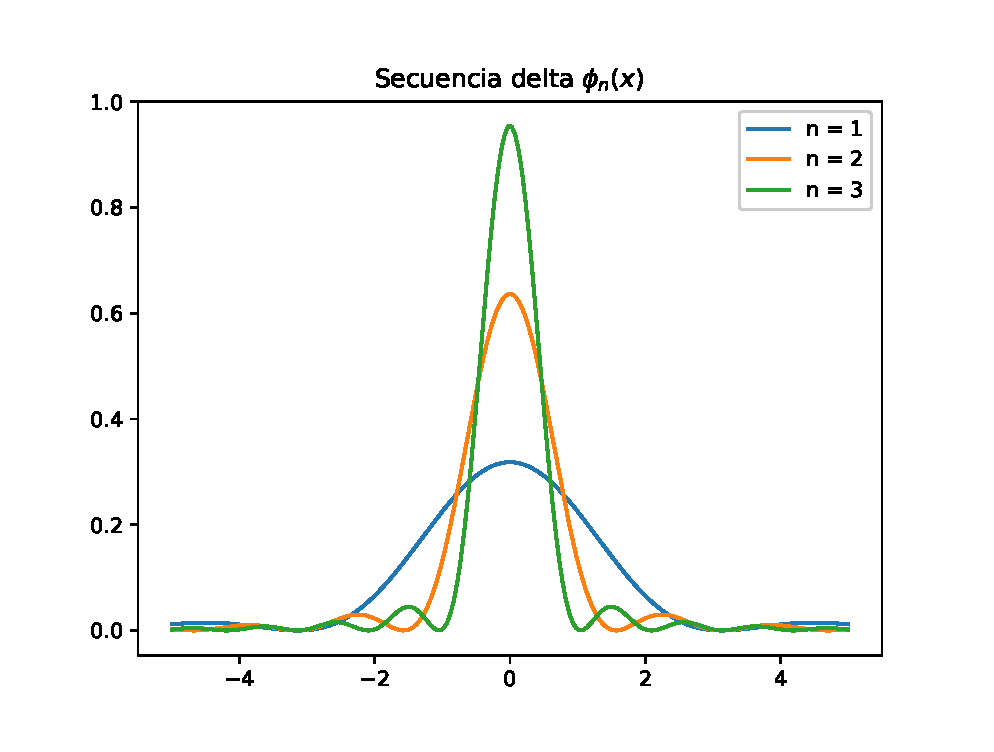
\includegraphics[scale=0.8]{Imagenes/secuencia_delta_03.eps}
%     \caption{Secuencia para $\phi_{n}$ con una función $\sin^{2}(x)/x$}
%     \label{fig:plot_secuencia_03}
% \end{figure}



% Tomemos en cuenta que no es correcto expresar que éstas secuencias convergen a la función delta: los límites de esas secuencias \emph{no existen} (de acuerdo a las definiciones conocidas de convergencia).

% Todas estas funciones están normalizadas a la unidad
% \begin{equation}
% \lim_{n \to \infty} \int_{- \infty}^{+ \infty} \phi_{n}(x) \: \dd{x} = 1
% \label{eq:ecuacion_delta_05}
% \end{equation}

% \subsection{Propiedades de la delta de Dirac.}

% Una vez que hemos definido la delta de Dirac, nos gustaría saber ahora como operar con y en ella. ¿Es posible decir algo sobre su derivada? La respuesta a esta pregunta es afirmativa y las secuencias delta hechas de funciones diferenciables nos permiten responder a la pregunta de manera precisa.
% \par
% Por ejemplo, sea la secuencia delta
% \begin{align*}
% \phi_{n} &= \dfrac{n}{\sqrt{\pi}} e^{-n^{2} x^{2}}
% \end{align*}
% entonces, al diferenciar la secuencia
% \begin{align*}
% \dv{\phi_{n}(x)}{x} = - \dfrac{2 \: n^{3}}{\sqrt{\pi}} \: x \: \exp(-n^{2} \: x^{2})
% \end{align*}
% \begin{figure}[H]
%     \centering
%     \includegraphics[scale=0.8]{Imagenes/secuencia_delta_04.eps}
%     \caption{Derivada de la secuencia delta.}
%     \label{fig:fig_figura_delta_04}
% \end{figure}
% Consideremos ahora la integral
% \begin{align*}
% \int_{-\infty}^{+\infty} \dv{\phi_{n}(x)}{x} \: f(x) \dd{x}
% \end{align*}
% donde $f(x)$ es diferenciable. Integrando por partes, se obtiene
% \begin{align*}
% \int_{-\infty}^{+\infty} \dv{\phi_{n}(x)}{x} \: f(x) \dd{x} = \phi_{n} \: f(x) \eval_{-\infty}^{+\infty} - \int_{-\infty}^{+\infty} \phi_{n} \: \dv{f(x)}{x} \dd{x}
% \end{align*}
% Suponemos que
% \begin{align*}
% \lim_{n \to \infty} \left( \dfrac{n}{\sqrt{\pi}} \right) \exp(-n^{2} \: x^{2}) \: f(x) = 0
% \end{align*}
% Esto normalmente es cierto, ya que estamos considerando funciones para las cuales la integral
% \begin{align*}
% \int_{-\infty}^{+\infty} \phi_{n}(x) \: f(x) \dd{x} 
% \end{align*}
% converge.
% \par
% Entonces, haciendo que $n \to \infty$, tenemos
% \begin{align*}
% \lim_{n \to \infty} \int_{-\infty}^{+\infty} \dv{\phi_{n}(x)}{x} \: f(x) \dd{x} = - \lim_{n \to \infty} \phi_{n}(x) \: f^{\prime} (x) \dd{x} =  -f^{\prime}(0)
% \end{align*}
% Vemos entonces que la secuencia $\phi^{\prime}(x)$ está relacionada con la propiedad de filtro.
% \begin{propiedad}

% La delta de Dirac satisface varias propiedades y conocerlas es de mucha utilidad cuando resolvemos problemas específicos en física. 
% \par

\section{Introduciendo más variables}
\frame[allowframebreaks]{\frametitle{Temas a revisar} \tableofcontents[currentsection, hideothersubsections]}
\subsection{Ampliando el uso de la delta}

\begin{frame}
\frametitle{Cambiando las variables}
Será muy común utilizar la delta de Dirac cuando tengamos más variables, \pause por lo que es conveniente representar la $\delta (x)$ en el correspondiente sistema.
\end{frame}
\begin{frame}
\frametitle{Introduciendo más variables}
\begin{align*}
\delta (\va{\bm{r}} - \va{\bm{r_{0}}}) = \delta (x - x_{0}) \: \delta (y - y_{0}) \: \delta (z - z_{0})
% \label{eq:ecuacion_A_03}
\end{align*}
\pause
de manera que al integrar sobre todo el espacio tenemos:
\pause
\begin{align*}
\scaleint{6ex} \delta (\va{\bm{r}} - \va{\bm{r_{0}}}) \: \dd{x} \dd{y}  \dd{z} = 1
\end{align*}
\end{frame}
\begin{frame}
\frametitle{Ejemplo con más variables}
La función delta permite especificar la densidad de carga debida a un conjunto de $N$ cargas puntuales de valores $q_{i}$ situadas en posiciones $\va{r_{i}}$ como:
\pause
\begin{align*}
\rho (\va{r}) = \nsum_{i=1}^{N} q_{i} \: \delta(\va{r} - \va{r_{i}})
% \label{eq:ecuacion_A_04}
\end{align*}
\end{frame}
\begin{frame}
\frametitle{Ejemplo con más variables}
Las propiedades de la función delta permiten obtener el potencial $\varphi(\va{r})$ evaluando la función dentro de la integral en los puntos $\va{r_{i}}$, es decir:
\pause
\begin{eqnarray*}
\begin{aligned}
\varphi(\va{r}) &= \scaleint{6ex} \dfrac{\rho(\va{r^{\prime}})}{\abs{\va{r} - \va{r^{\prime}}}} \: d^{3}r^{\prime} = \pause \nsum_{i=1}^{N} q_{i} \scaleint{6ex} \dfrac{\delta ( \va{r} - \va{r_{i}})}{\abs{\va{r} - \va{r^{\prime}}}} \: d^{3}r^{\prime} = \\[0.5em] \pause
&= \nsum_{i=1}^{N} \dfrac{q_{i}}{\abs{\va{r} - \va{r_{i}}}}
% \label{eq:ecuacion_A_05}
\end{aligned}
\end{eqnarray*}
\end{frame}
\begin{frame}
\frametitle{Ejemplo con más variables}
Nótese que $\delta (x)$ tiene unidades de inverso de $x$ y $\delta (\va{r})$ tiene unidades de densidad numérica.
\end{frame}
\begin{frame}
\frametitle{La $\delta (x)$ en otras geometrías}
La $\delta (x)$ toma una forma particular en coordenadas cilíndricas y esféricas, dadas por la condición de normalización:
\pause
\setbeamercolor{item projected}{bg=ao,fg=white}
\setbeamertemplate{enumerate items}{%
\usebeamercolor[bg]{item projected}%
\raisebox{1.5pt}{\colorbox{bg}{\color{fg}\footnotesize\insertenumlabel}}%
}
\begin{enumerate}
\item Para coordenadas cilíndricas:
\begin{align*}
\begin{aligned}
&\scaleint{6ex} \delta (\va{r} - \va{r}_{0}) \: R \: \dd{R} \: \dd{\varphi} \: \dd{z} \\[0.5em]
&\Rightarrow \delta (\va{r}) =  \dfrac{1}{R} \: \delta (R {-} R_{0}) \: \delta (\varphi {-} \varphi_{0}) \: \delta (z {-} z_{0})
\end{aligned}
\end{align*}
\seti
\end{enumerate}
\end{frame}
\begin{frame}
\frametitle{La $\delta (x)$ en otras geometrías}
\setbeamercolor{item projected}{bg=ao,fg=white}
\setbeamertemplate{enumerate items}{%
\usebeamercolor[bg]{item projected}%
\raisebox{1.5pt}{\colorbox{bg}{\color{fg}\footnotesize\insertenumlabel}}%
}
\begin{enumerate}
\conti
\item Para coordenadas esféricas:
\begin{align*}
\begin{aligned}
&\scaleint{6ex} \delta (\va{r} - \va{r}_{0}) \: r^{2} \, \dd{r} \, \sin \theta \, \dd{\theta} \, \dd{\varphi} = 1 \\
&\Rightarrow \delta (\va{r}) = \dfrac{1}{r^{2}} \: \delta (r {-} r_{0}) \, \delta (\cos \theta {-} \cos \theta_{0}) \, \delta (\varphi {-} \varphi_{0})
\end{aligned}
\end{align*}
\end{enumerate}
\end{frame}
% Algunas funciones generan en el límite la función delta:
% \begin{align*}
% \delta(x) = \begin{cases}
% \displaystyle
% \lim_{\varepsilon \to 0^{+}} \dfrac{1}{\pi} \, \dfrac{\varepsilon}{x^{2} + \varepsilon^{2}} & \mbox{Lorentz} \\[1em]
% \displaystyle
% \lim_{\sigma \to 0^{+}} \dfrac{1}{\sigma \, \sqrt{2 \, \pi}} \, \exp \left( - \dfrac{x^{2}}{2 \, \sigma^{2}} \right) & \mbox{Gaussiana} \\[1em]
% \displaystyle \lim_{\varepsilon \to 0^{+}} \dfrac{\sin(x / \varepsilon)}{ \pi \, x} & \mbox{Dirichlet} \\[1em]
% \displaystyle \lim_{L \to \infty} \dfrac{1}{2 \, \pi} \int_{- \abs{L}}^{\abs{L}} \exp(i \, k \, x) \dd{k} & \mbox{Fourier}
% \end{cases}
% \end{align*}
% \section*{Ejercicios a cuenta}
% \begin{enumerate}[label=\roman*.]
% \item Demuestra que 
% \[ \nabla \vdot \left( \dfrac{e_{r}}{r^{2}} \right) = 0 \hspace{1cm} \mbox{para } r > 0 \]
% Tip: Se puede resolver en coordenadas cartesianas, pero es más fácil usando coordenadas esféricas.
% \item Demuestra que 
% \[ \nabla \left( \dfrac{1}{r} \right) = - \dfrac{e_{r}}{r^{2}} \]
% \end{enumerate}
\end{document}